\documentclass{report}
\usepackage{graphicx} % Required for inserting images
\usepackage[italian]{babel}
\usepackage{tikz}
\usepackage{hyperref}
\usepackage{amsmath}
\usepackage{xcolor}
\usepackage{float}

\definecolor{darkgreen}{rgb}{0.0, 0.5, 0.0}


\title{Mano e Palmo - Biometria a contatto}
\date{Parte VII}

\begin{document}

\maketitle

\tableofcontents
\newpage

\chapter{Introduzione}

\begin{itemize}
    \item È un tratto biometrico \textbf{molto ben accettato dagli utenti}
    in quanto poco invasivo
    \item È una tecnologia matura (presente dal 1979)
    \item Offre un \textbf{discreto livello di accuratezza} senza dover 
    chiedere all'utente sample critici per la privacy (come impronta o iride)
    \item Offre la \textbf{possibilità di funzionare in modo multimodale} controllando 
    più aspetti come immagini, misure, pattern delle vene
    \item Buona diffusione sul mercato
\end{itemize}

\section{Applicazioni}
\begin{itemize}
    \item L'utente deve essere collaborativo
    \item I sistemi possono essere centralizzati, coprendo gli accessi
    a grandi aree (aeroporto, basi militari, \dots)
    \item Sistemi usati principalmente per il \textbf{controllo degli accessi} o per \textit{\textbf{time and attendace}} (controllo presenze sui luoghi di lavoro)
    \item Preferita dal nostro \textbf{\textit{Garante della Privacy}}
\end{itemize}

\section{Vantaggi e Svantaggi}
\begin{itemize}
    \item \textcolor{darkgreen}{\textbf{Vantaggi}}
    \begin{itemize}
        \item Tecnologia consolidata
        \item Sensore robusto 
        \item Dimensioni template ridotte 
        \item Minore impatto su privacy degli utenti 
    \end{itemize}
    \item \textcolor{red}{\textbf{Svantaggi}}
    \begin{itemize}
        \item Costo 
        \item Dimensioni e peso 
        \item Sensibilità a luce diurna
    \end{itemize}
\end{itemize}

\section{Sensori}
I sensori di solito lavorano su tre viste:
\begin{itemize}
    \item palmare 
    \item laterale 
    \item dorsale
\end{itemize}

\subsection{\textit{Pegs or Pegs-free}}
In commercio esistono dei dispositivi con dei pioli per il corretto 
posizionamento delle mani, ed altri senza.

$\rightarrow$ con i pioli il sistema diventa più accurato, perché viene 
ridotta la variabilità intraclasse del sample  

\begin{figure}[ht]
    \centering
    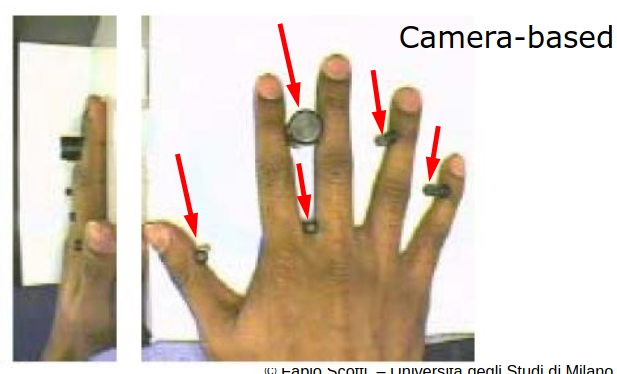
\includegraphics[width=1\linewidth]{images/pioli.png}
\end{figure}




\chapter{Matching}

\section{Alcuni tipi delle 90 features estraibili}
\begin{figure}[ht]
    \centering
    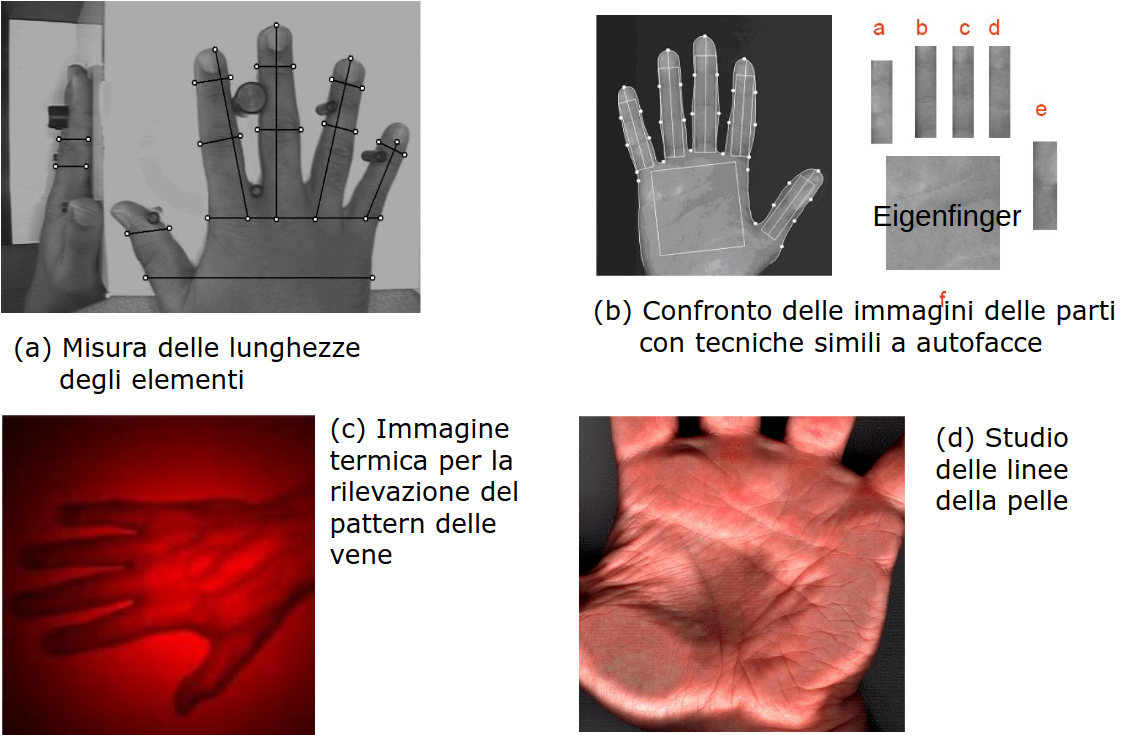
\includegraphics[width=1\linewidth]{images/features.png}
\end{figure}

\newpage
\section{Passi per il matching}
\begin{enumerate}
    \item \textbf{Peg removal:} conoscendo la posizione fissa dei 
    pioli è facile sottrarli alle immagini 
    \item \textbf{Estrazione dei contorni:} viene segmentata l'immagine 
    e trovato il contorno esterno della mano

    \begin{figure}[ht]
        \centering
        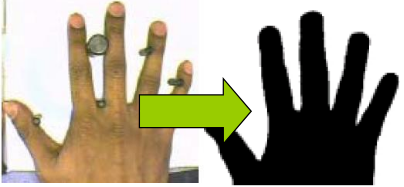
\includegraphics[width=0.6\linewidth]{images/contorni.png}
    \end{figure}
    \item \textbf{Estrazione delle dita ed allineamento:} le 5 dita 
    vengono estratte dal profilo ed allineate seperatamente a partire da posizioni 
    standard; questo velocizza il processo di matching

    \begin{figure}[ht]
        \centering
        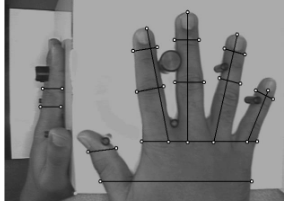
\includegraphics[width=0.5\linewidth]{images/allineamento.png}
    \end{figure}
    \item \textbf{Matching:}
    \begin{itemize}
        \item le curve delle mani da confrontare vengono trasformate in una 
        serie di punti 
        \item il matching lavora individuando le coppie di punti e misurando 
        la loro distanza

        \noindent$\rightarrow$ se la distanza media (MAE, \textit{Mean Alignement Error}) è minore di una certa soglia 
        l'utente è considerato genuino, altrimeniti come un impostore
    \end{itemize}
    \begin{figure}[ht]
        \centering
        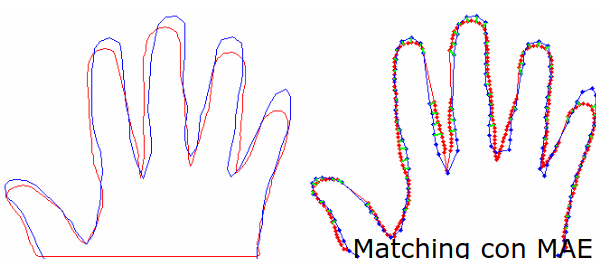
\includegraphics[width=1\linewidth]{images/matching.png}
    \end{figure}
\end{enumerate}

\newpage
\section{\textit{Eigenfingers}}
In un modo simile al metodo delle autofacce, da un database 
di immagini di mani è possibile ricostruire le dita e il palmo.





\end{document}